\chapter{RD53Aの回路図とフレキシブル基板} \label{chap:rd53a_circit}

\begin{figure}[bpt]
  \begin{center}
    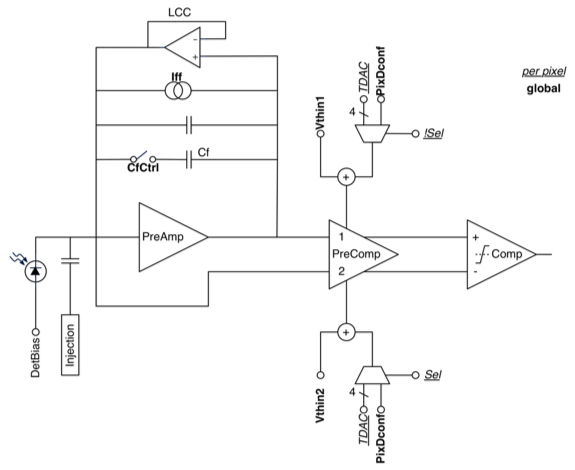
\includegraphics[width=8cm]{diff_fe}
    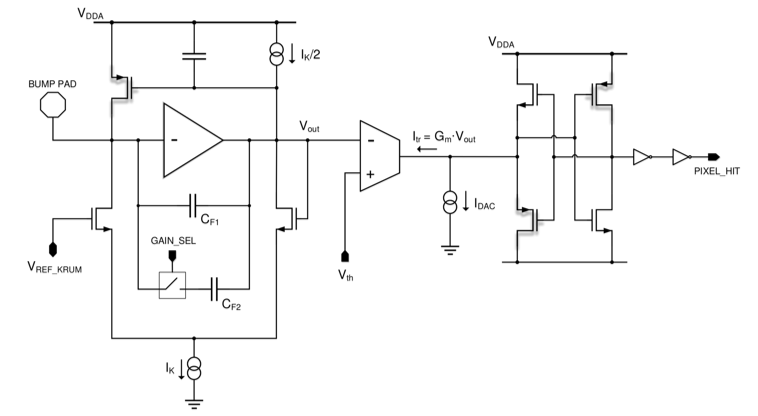
\includegraphics[width=8cm]{lin_fe}
    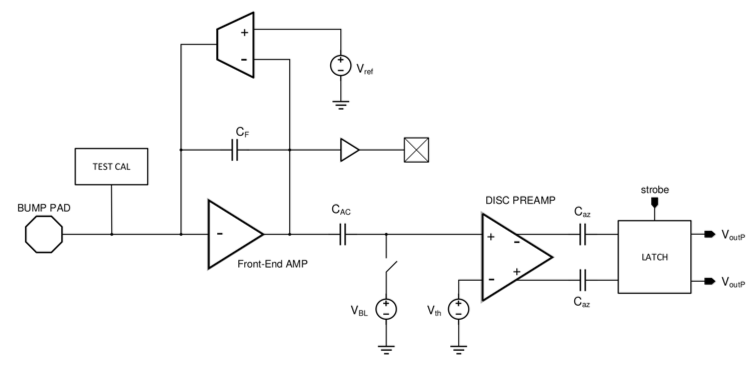
\includegraphics[width=8cm]{syn_fe}
  \caption[アナログフロントエンド]{アナログフロントエンド\cite{2-1}}
  \label{analog_fe}
  \end{center}
\end{figure}

\begin{figure}[bpt]\centering
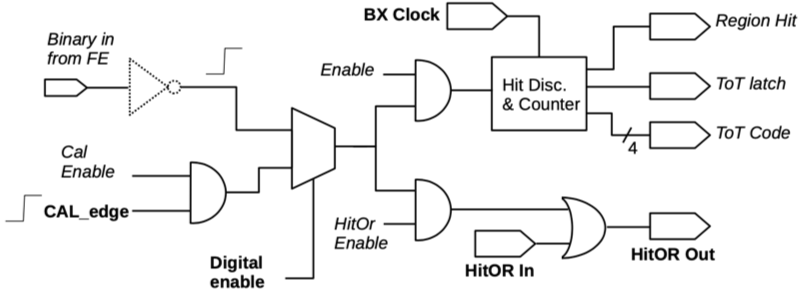
\includegraphics[width=10cm]{digital_fe}
\caption[デジタルフロントエンド]{デジタルフロントエンド\cite{2-1}}
\label{digital_fe}
\end{figure}

\begin{figure}[bpt]\centering
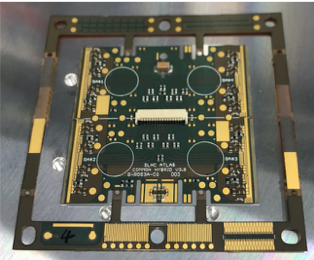
\includegraphics[width=10cm]{pcb}
\caption[フレキシブル基板]{フレキシブル基板}
\label{pcb}
\end{figure}


